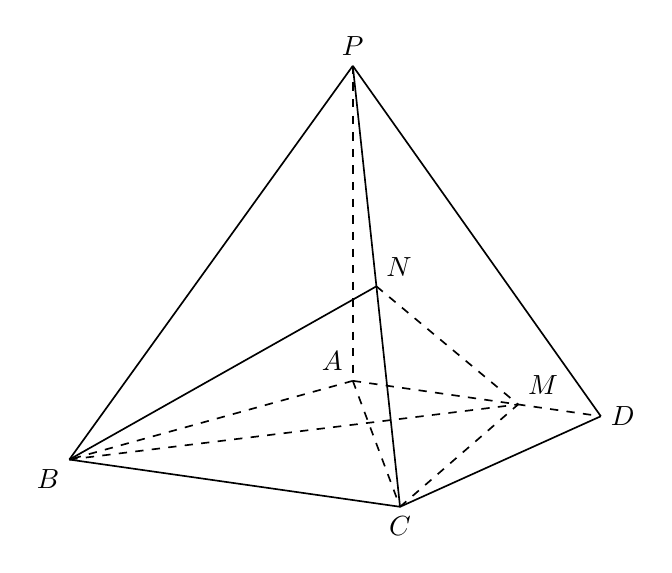
\begin{tikzpicture}[line width=0.6pt, font=\normalsize]
% 四棱锥 P-ABCD 示意（透视示意，非度量投影）
\coordinate (P) at (0,4.6);
\coordinate (A) at (0,0.6);
\coordinate (B) at (-3.6,-0.4);
\coordinate (C) at (0.6,-1.0);
\coordinate (D) at (3.15,0.15);
\coordinate (M) at (2.1,0.3);
\coordinate (N) at (0.3,1.8);
% 可见棱（实线）
\draw (P) -- (B);
\draw (P) -- (N) -- (C);
\draw (P) -- (D);
\draw (B) -- (C);
\draw (C) -- (D);
\draw (B) -- (N);
% 遮挡棱（虚线）
\draw[dashed] (P) -- (A);
\draw[dashed] (A) -- (B);
\draw[dashed] (A) -- (M) -- (D);
\draw[dashed] (B) -- (M);
\draw[dashed] (A) -- (C);
\draw[dashed] (N) -- (M);
\draw[dashed] (C) -- (M);
% 标签
\node[above] at (P) {$P$};
\node[above left] at (A) {$A$};
\node[below left] at (B) {$B$};
\node[below] at (C) {$C$};
\node[right] at (D) {$D$};
\node[above right] at (M) {$M$};
\node[above right] at (N) {$N$};
\end{tikzpicture}
